\chapter{Avaliação dos Extratores de Tópicos}\label{cap-extratores}

% Dar uma geral nesse primeiro parágrafo
	% Escolha dos Algorítmos
	% Escolha do método de avaliação (subjetivo com questionario)

% -- 1 - Motivação para o experimento.
Nesse capítulo, as técnicas de extração de tópicos são analisadas. O objetivo é comparar os algoritmos de extração de tópicos na tarefa de extração de padrões no contexto das atas de reunião no que tange a qualidade dos agrupamentos e seus descritores bem como sua capacidade de representar os segmentos. Para essa análise, escolheu-se os modelos LDA, PLSA e K-Means devido a popularidade desses métodos os quais são amplamente utilizados~\cite{DZhu20122} e frequentemente referenciados em trabalhos voltados a organização de bases textuais~\cite{Aggarwal2018, OCallaghan2015, Steyvers2007}.
Os algoritmos foram inicialmente configurados com base em avaliações internas~\cite{Hassani2017} e observações empíricas nas quais escolheu-se os melhores valores para seus parâmetros. Os resultados desses modelos foram submetidos a uma avaliação subjetiva a fim de analisá-los junto a usuários com afinidade com atas de reuniões. 

Nessa avaliação, a técnica de segmentação textual também foi avaliada, uma vez que é a etapa anterior a extração de tópicos está diretamente ligada a os resultados apresentados ao avaliador bem como pode interferir no funcionamento dos modelos de extração de tópicos. Assim, a técnica de segmentação textual foi avaliada subjetivamente em complemento a análise estatística apresentada no Capítulo~\ref{cap-segmentadores}.

A avaliação se deu por meio de questionários onde profissionais com afinidade com atas de reunião forneceram suas percepções em relação aos resultados dos modelos de extração de tópicos. Por fim, os dados obtidos dos experimentos serviram de base para as análises dos algoritmos e de sua aplicação no contexto das atas de reuniões.
% os dados serviram como base para análise dos algoritmos 

\section{Configuração experimental}

% A qtd de tópicos é um parametro importante.  % Todos com 70 tópicos e 5 extratores;
Durante os primeiros testes, a qualidade dos resultados mostrou-se sensível à quantidade de tópicos extraídos.
Inicialmente, realizou-se um teste prévio utilizando uma versão não-paramétrica dos algorítimos a fim de automaticamente obter valores ótimos para esse parâmetro por meio da análise das medidas Silhueta e Coesão. Essa configuração automática resulta valores em torno de 20 tópicos. Contudo, os resultados apresentam grupos com muitos segmentos (em torno de 100) o que os tornam pouco coesos em relação a um assunto central, além de diminuir a capacidade representativa dos descritores.
Com base em observações empíricas, verificou-se que valores abaixo de 60 tópicos geram grupos com muitos segmentos o que por consequência torna os grupos menos coesos por incluir segmentos com assuntos muito distantes. Por outro lado, valores acima de 80 geram tópicos com poucos segmentos, permitindo que assuntos próximos sejam atribuídos a grupos distintos. Nesse trabalho, optou-se por configurar os algoritmos para extrair 70 tópicos da coleção de segmentos por apresentar uma distribuição mais coerente em termos de agrupamento na visão de usuário.

Outro fator importante é a quantidade de descritores selecionados para cada tópico. Com base no experimento de anotações em segmentação, descrito no Capítulo~\ref{cap-segmentadores}, os anotadores selecionaram em média 5 palavras para descrever os segmentos, sendo esse valor adotado para essa avaliação.




\section{Critérios de avaliação}

% - Explicar que foram 2 consultas (quais) e mostrar os extratores.
% - 4 - Procedimento (2 consultas, técnicas em ordens diferentes).
Após a identificação da configuração mais adequada para cada algoritmo, cada um dos modelos de extração de tópicos foi submetido a duas consultas\footnote{O termo consulta significa um conjunto de palavras chave passadas à um sistema de busca.}: ``\textit{compra de equipamentos}'' e ``\textit{defesa de dissertação}'' gerando 6 cenários distintos a serem analisados. 
Para cada cenário, o sistema seleciona o tópico com maior relevância com a consulta e em seguida exibe 5 segmentos desse tópico escolhidos aleatoriamente. 
Vale dizer que nessa avaliação as técnicas de ranqueamento dos resultados não são aplicadas para que estas não interfiram na avaliação dos extratores, contudo, o sistema final poderá ranquear também os segmentos com maior relevância de um ou mais tópicos por meio de técnicas de recuperação de informação. 
Os resultados desses cenários foram apresentados a um grupo de avaliadores que individualmente avaliaram a qualidade das técnicas de extração de tópicos. 
%

% -- 3 - Escolha dos participantes.
O perfil dos avaliadores é de profissionais da area acadêmica/escolar devido à sua afinidade com o ambiente de gestão e conhecimentos de assuntos relacionados ao \textit{corpus} estudado nesse trabalho. O grupo convidado a participar do experimento é formado por 24 profissionais da UFSCar campus Sorocaba, 13 profissionais de escolas técnicas e 3 profissionais de escolas do Ensino Fundamental, sendo 12 ocupantes de cargos de gestão como coordenadores de curso e diretores, 17 membros de conselhos, 5 profissionais administrativos e 3 professores, totalizando 41 avaliadores em que a maioria afirma ter afinidade com atas e reuniões. Apenas 3 declararam nenhuma afinidade com esses documentos, sendo esses últimos descartados por não se adequarem ao perfil desejado. Os avaliadores foram divididos em dois grupos, sendo o primeiro formado por 18 participantes que avaliaram a primeira consulta, ``\textit{compra de equipamentos}'' e o segundo formado por 19 participantes que avaliaram a segunda consulta, ``\textit{defesa de dissertação}''. Os grupos avaliaram as técnicas de extração tópicos a partir de uma consulta, ou seja, cada indivíduo avaliou 3 cenários distintos. A avaliação consistiu de um documento impresso contendo uma breve apresentação do trabalho, seguido de uma cópia dos resultados das técnicas de extração de tópicos. Para cada técnica, os avaliadores recebiam 4 questões sobre os resultados. Os documentos de ambas avaliações podem ser vistas no Anexo~\ref{anexo:avaliacoes}.

% X profissionais de gestão de instituições 

% -- 2 - Escolha das questões.
O questionário foi formado por questões envolvendo aspectos os extratores de tópicos e questões referentes à técnica de segmentação textual empregada.
As respostas seguiram a escala \textit{Likert}~\cite{Norman2010} com 5 alternativas. 
% , conforme mostrado:

% \begin{enumerate}
	% \item Todos os trechos apresentados compartilham um mesmo assunto.
	% \item As palavras \textit{<descritores>} resumem bem o assunto tratado nos trechos.
	% \item Existem trechos que não tratam de um único assunto?
	% \item Existem trechos incompletos e insuficientes para compreensão do assunto do trecho?
% \end{enumerate}


As questões 1 e 2 estão relacionadas ao extrator de tópicos. 
A primeira, \textit{``Todos os trechos apresentados compartilham um mesmo assunto.''}, refere-se ao agrupamento dos segmentos pela qual foi avaliada a semelhança dos trechos em termos de assunto. 
A segunda questão, \textit{``As palavras \textit{<descritores>} resumem bem o assunto tratado nos trechos.''}, diz respeito aos descritores selecionados, ao respondê-la o avaliador indicou o quão bem esses termos representam aquele grupo.
As questões 3 e 4 estão ligadas à técnica de segmentação utilizada, o BayesSeg conforme já mencionado no Capítulo~\ref{cap-segmentadores}. 
A questão 3, \textit{``Existem trechos que não tratam de um único assunto?''}, diz respeito à coesão de cada segmento, levando em conta a homogeneidade do texto em relação a um assunto. A questão 4, \textit{``Existem trechos incompletos e insuficientes para compreensão do assunto do trecho?''}, refere-se a completude dos segmentos, ou seja, o quão bem os segmentos podem ser bem compreendidos independentemente da leitura do documento integral.
Para afastar a hipótese de que os resultados das técnicas fossem influenciados pela ordem apresentada, essas foram apresentadas aos avaliadores em ordem aleatórias.
% -- 5 - Escolha dos temas para consulta: 




% A primeira refere-se ao agrupamento dos segmentos pela qual foi avaliada a semelhança dos trechos em termos de assunto.

\section{Avaliação dos Extratores junto a Usuários}
% \section{Resultados}

% -- Quantitativos
Inicialmente, a coleção de documentos utilizada como base nesse experimento foi constituída de 175 atas, dessas, foram extraídos 1272 segmentos dos quais os algoritmos atribuíram em média 19 segmentos a cada tópico. Na Tabela~\ref{tab:segquanti} é exibido para cada cenário a quantidade de segmentos atribuídos ao tópico seleciona na busca, bem como os descritores que os identificam.
 
\begin{table}[!h]
\begin{tabular}{|c|c|l|c|}
 \hline 
 \textbf{Consulta} &\textbf{Algoritmo }& \textbf{Descritores }& \textbf{\#Seg} \\ \hline
 \multirow{3}{*}{Consulta 1} &
 KMeans & \textit{compra, material, verba, permanente e valor} & 13 \\  \cline{2-4} 
 & LDA    & \textit{verba, compra, pagamento, material e valor}  & 47 \\  \cline{2-4}
 & PLSA   & \textit{verba, compra, pagamento, valor e realizada} & 9  \\  \hline 
 \multirow{3}{*}{Consulta 2} &
 KMeans & \textit{orientada, meses, defesa, prazo e dissertação} & 12 \\  \cline{2-4}
 & LDA    & \textit{aprovado, defesa, pedido, dissertação e orientada} & 19 \\ \cline{2-4} 
 & PLSA   & \textit{orientada, prazo, bolsa, meses e defesa} & 19 \\  \hline 
 \end{tabular}  
 \label{tab:segquanti}
 \caption{Descritores e número de segmentos no tópico selecionado pelos Algoritmos}
\end{table} 

Na primeira consulta, \textit{``compra de equipamentos''},  os 3 algoritmos selecionaram um total de 22 segmentos diferentes, sendo que desses 12 foram concomitantemente selecionados por todos os algoritmos e o LDA e o PLSA compartilham 3 desses segmentos nos resultados.
Na segunda  consulta, \textit{``defesa de dissertação''}, os 3 algoritmos selecionaram um total de 49 segmentos diferentes, sendo que desses 4 foram selecionados concomitantemente por todos os algoritmos. O K-Means compartilha 7 segmentos com o LDA e 3 com o PLSA. O LDA e o PLSA compartilham 2 segmentos nos resultados.
% --> E daí?



Nessa seção, os dados coletados das avaliações são apresentados e analisados. Os modelos de extração de tópicos discutidos nesse trabalho são comparados de acordo com os critérios mencionados anteriormente: 
(1) comparar algoritmos de extração de tópicos na tarefa de extração de padrões no contexto das atas de reunião, 
% (2) analisar a qualidade dos agrupamentos no que tange a navegação por grupos com mesmo tópico, 
(2) analisar a qualidade dos descritores extraídos para recuperar os documentos dos grupos.
Além disso, as questões referentes à segmentação, são analisadas a fim de 
% (3) 
validar a performance do segmentador empregado, como complemento ao experimento discutido na Seção~\ref{cap-segmentadores}.


Na Figura~\ref{fig:Q1} é apresentado as frequência das respostas coletadas sobre a primeira questão, \textit{``Todos os trechos apresentados compartilham um mesmo assunto.''}, a qual refere-se a qualidade do agrupamento levando em conta a semelhança dos segmentos em termos de assunto. A afirmação foi dado como opções de resposta: 
\textit{``Discordo Totalmente''}; 
\textit{``Discordo Parcialmente''}; 
\textit{``Não Concordo, nem Discordo''}; 
\textit{``Concordo Parcialmente''} e 
\textit{``Concordo Totalmente''}, 
representadas na figura como DT, DP, NCND e CT, respectivamente.
Verifica-se que o K-Means tem resultados similares ao LDA enquanto o PLSA se mostrou menos eficiente nesse critério uma vez que mais avaliadores rejeitaram a afirmação de que todos os segmentos tratam de um único assunto em comum. 

\begin{figure}[!h] \centering     %%% not \center
%	\subfigure{ \label{fig:kmeans}
		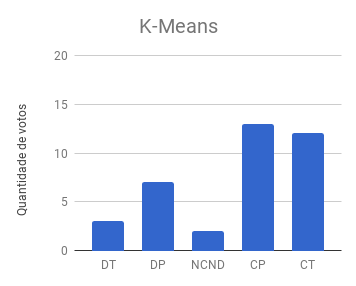
\includegraphics[width=.31\textwidth]{conteudo/capitulos/figs/figuras-experimento/Q1-KMeans.png}
%	}	
%	\subfigure{ \label{fig:lda}
		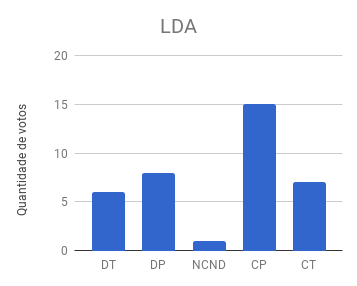
\includegraphics[width=.31\textwidth]{conteudo/capitulos/figs/figuras-experimento/Q1-LDA.png}
%	}
%	\subfigure{ \label{fig:plsa}
		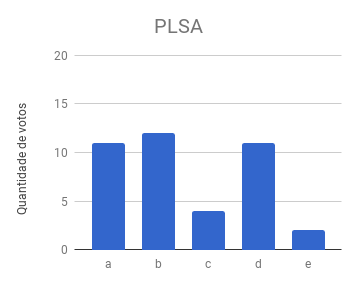
\includegraphics[width=.31\textwidth]{conteudo/capitulos/figs/figuras-experimento/Q1-PLSA.png}
%	} 
	\caption{Contagem de respostas referente a primeira questão em que o eixo vertical indica a frequência das alternativas.  }
	\label{fig:Q1}
\end{figure}

% A segunda questão diz respeito aos descritores selecionados, ao respondê-la o avaliador indicou o quão bem esses termos representam aquele grupo.
Outro ponto importante a ser analisado é a capacidade representativa dos descritores, ou seja, o quão bem os descritores podem representar o tópico ao qual os segmentos foram atribuídos. A Figura~\ref{fig:Q2} contém a frequência as respostas referentes a segunda questão, \textit{``As palavras \textit{<descritores>} resumem bem o assunto tratado nos trechos.''} onde os avaliadores tiveram as mesmas opções de respostas que a anterior. Observa-se na Figura~\ref{fig:Q2} que no caso do K-Means a quantidade de usuários que concordam com a afirmação de que os descritores extraídos são bons atributos para descrever o teor dos segmentos foi bem maior em relação ao que discordam.

\begin{figure}[!h] \centering     %%% not \center

%	\subfigure{ \label{fig:kmeans}
		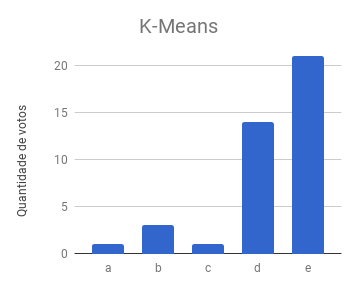
\includegraphics[width=.31\textwidth]{conteudo/capitulos/figs/figuras-experimento/Q2-KMeans.png}
%	}	
%	\subfigure{ \label{fig:lda}
		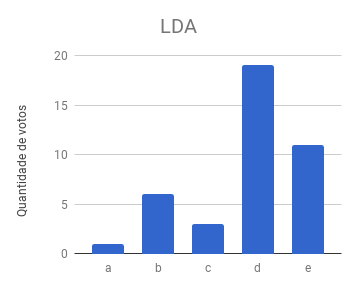
\includegraphics[width=.31\textwidth]{conteudo/capitulos/figs/figuras-experimento/Q2-LDA.png}
%	}
%	\subfigure{ \label{fig:plsa}
		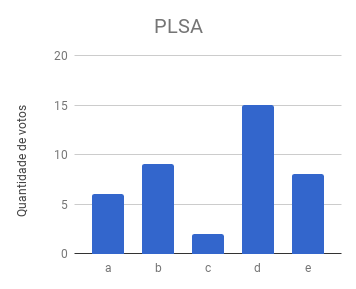
\includegraphics[width=.31\textwidth]{conteudo/capitulos/figs/figuras-experimento/Q2-PLSA.png}
%	}
	\caption{Contagem de respostas referente a segunda questão em que o eixo vertical indica a frequência das alternativas.  }
	\label{fig:Q2}
\end{figure}


% -- Conclusão : extração de padrões	
Ao analisar os resultados, verifica-se que de maneira geral os modelos K-Means e LDA podem ser considerados satisfatórios na tarefa de agrupar e representar os segmentos das atas.
Verifica-se também que para o modelo K-Means os avaliadores identificaram que, na maioria dos casos, houve resultados satisfatórios, principalmente quanto a representatividade dos descritores. Embora a avaliação aponte imperfeições, esse modelo apresenta maior uniformidade em relação aos demais.

\section{Validação do Segmentador}
% -- Lalazinho

Nessa seção, os dados coletados no experimento são utilizados para validar o segmentador empregado nesse trabalho. O algoritmo \textit{BayesSeg} é analisado quanto a sua capacidade de extrair segmentos coesos, isto é, que tratem de um único assunto central evitando trazer informações alheias ou irrelevantes. Outro critério avaliado é a completude dos segmentos, ou seja, o segmentos devem conter informação suficiente para o entendimento do texto sem necessidade de outro texto adjacente. Em outras palavras, usuário deve receber informações precisas sobre o tópico selecionado.

Os dados coletados de ambas consultas foram somadas, uma vez que esta é uma etapa anterior à extração de tópicos, a princípio, o modelo que selecionou os segmentos não interfere em sua avaliação. Assim, a Figura~\ref{fig:Q3} mostra as respostas do avaliadores considerando todos os cenários. As respostas referentes a terceira questão, na qual se averígua a homogeneidade de cada segmento quanto ao seu assunto central, apontam que poucos segmentos contém mais de um assunto.

\begin{figure}[!h] \centering     %%% not \center

		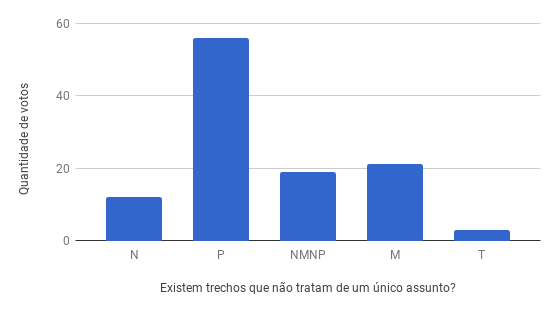
\includegraphics[width=.48\textwidth]{conteudo/capitulos/figs/figuras-experimento/Q3-Seg.png}
	\caption{Contagem de respostas referente a terceira questão em que o eixo vertical indica a frequência das alternativas.  }
	\label{fig:Q3}
\end{figure}


Ainda sobre a qualidade da segmentação, a Figura~\ref{fig:Q4} mostra os resultados da quarta questão a qual investiga a integridade de cada segmento, isto é, sua capacidade de informar o usuário sobre o assunto que trata sem necessidade de se recorrer a leitura do documento integral. Nesse critério, a maioria das avaliações indicam que nenhum ou poucos segmentos apresentam texto insuficiente para leitura.  Uma análise mais detalhada das questões relacionadas a segmentação das atas foi discutida no Capítulo~\ref{cap-segmentadores}, ficando aqui análises de pontos onde a segmentação influencia os extratores e os resultados finais apresentados ao usuário.


\begin{figure}[!h] \centering     %%% not \center

		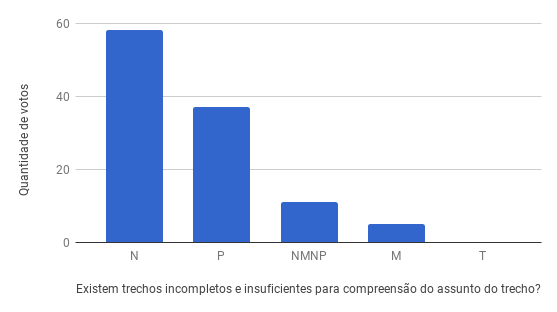
\includegraphics[width=.48\textwidth]{conteudo/capitulos/figs/figuras-experimento/Q4-Seg.png}
	\caption{Contagem de respostas referente a quarta questão em que o eixo vertical indica a frequência das alternativas.  }
	\label{fig:Q4}
\end{figure}


Outra questão analisada foi o comportamento dos modelos nas diferentes consultas. Ao se isolar as respostas das questões referentes a uma consulta específica, nota-se certa alteração nas respostas dos modelos. 
Os gráficos apresentados na Figura~\ref{fig:c12-q1}, mostram na primeira superior as respostas para cada modelo considerando-se os segmentos extraídos na primeira consulta e na linha inferior aqueles referentes a segunda consulta. O K-Means apresenta uma diminuição considerável na segunda consulta em relação a primeira no que se refere a respostas afirmando que os todos os segmentos compartilham um único assunto, e um aumento de respostam indicando discordância total com a afirmação da questão.
De forma semelhante, o PLSA apresenta diminuição de respostas positivas para essa afirmação e na proporção que há um aumento de respostas negativas. 
Por outro lado o LDA mantém resultados semelhantes em ambas as consultas, nas quais apresenta resultados equilibrados entre respostas positivas e negativas. Em outras palavras, os modelos K-Means e PLSA sofreram perda de desempenho enquanto o LDA manteve-se estável em ambas consultas.





\begin{figure}[!h] \centering     %%% not \center

%	\subfigure{ \label{fig:c1q1kmeans}
		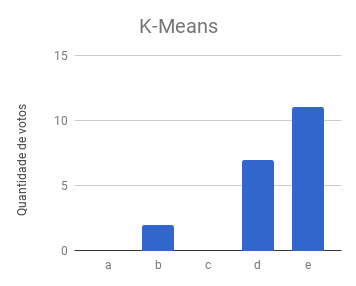
\includegraphics[width=.31\textwidth]{conteudo/capitulos/figs/figuras-experimento/C1-Q1-KMeans.png}
%	}	
%	\subfigure{ \label{fig:c1q1lda}
		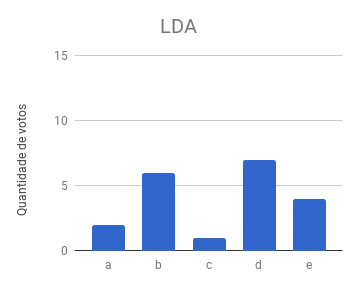
\includegraphics[width=.31\textwidth]{conteudo/capitulos/figs/figuras-experimento/C1-Q1-LDA.png}
%	}
%	\subfigure{ \label{fig:c1q1plsa}
		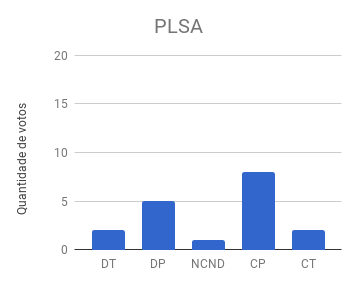
\includegraphics[width=.31\textwidth]{conteudo/capitulos/figs/figuras-experimento/C1-Q1-PLSA.png}
%	}
%	\subfigure{ \label{fig:c2q1kmeans}
		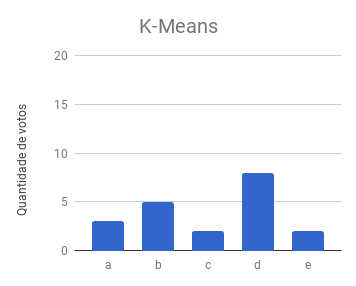
\includegraphics[width=.31\textwidth]{conteudo/capitulos/figs/figuras-experimento/C2-Q1-KMeans.png}
%	}	
%	\subfigure{ \label{fig:c2q1lda}
		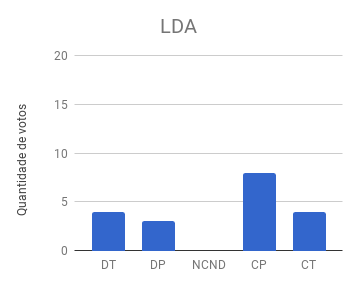
\includegraphics[width=.31\textwidth]{conteudo/capitulos/figs/figuras-experimento/C2-Q1-LDA.png}
%	}
%	\subfigure{ \label{fig:c2q1plsa}
		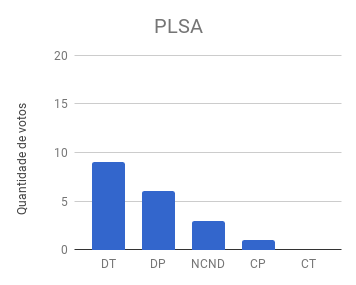
\includegraphics[width=.31\textwidth]{conteudo/capitulos/figs/figuras-experimento/C2-Q1-PLSA.png}
%	}

	\caption{Contagem das respostas referentes a Primeira questão. A primeira consulta, ``\textit{compra de equipamentos}'', é mostrada na linha superior e a segunda consulta, ``\textit{defesa de dissertação}'', na linha inferior.}
	\label{fig:c12-q1}
\end{figure}



Ao analisar separadamente a segunda questão, referente a representatividade dos descritores observa-se na Figura~\ref{fig:c12-q2} que todos os modelos apresentam perca de performance nesse critério, contudo, de forma acentuada no PLSA. 



\begin{figure}[!h] \centering     %%% not \center

%	\subfigure{ \label{fig:c1q2kmeans}
		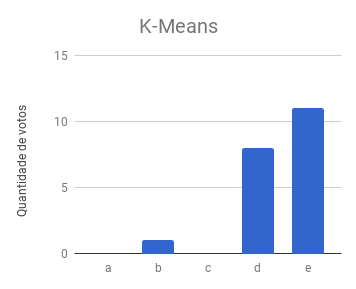
\includegraphics[width=.31\textwidth]{conteudo/capitulos/figs/figuras-experimento/C1-Q2-KMeans.png}
%	}	
%	\subfigure{ \label{fig:c1q2lda}
		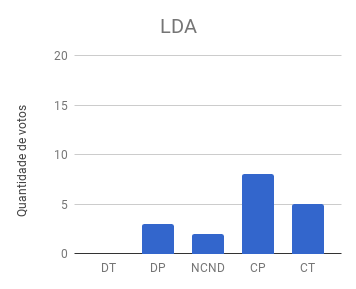
\includegraphics[width=.31\textwidth]{conteudo/capitulos/figs/figuras-experimento/C1-Q2-LDA.png}
%	}
%	\subfigure{ \label{fig:c1q2plsa}
		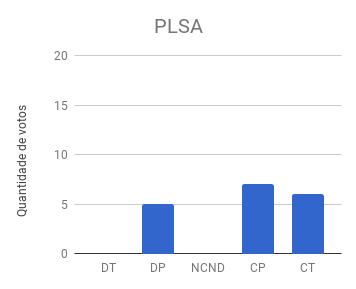
\includegraphics[width=.31\textwidth]{conteudo/capitulos/figs/figuras-experimento/C1-Q2-PLSA.png}
%	}
%	\subfigure{ \label{fig:c2q2kmeans}
		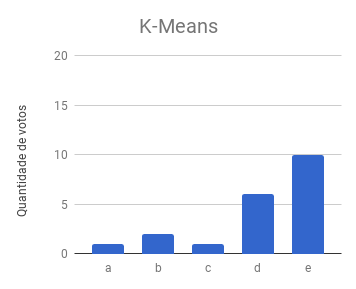
\includegraphics[width=.31\textwidth]{conteudo/capitulos/figs/figuras-experimento/C2-Q2-KMeans.png}
%	}	
%	\subfigure{ \label{fig:c2q2lda}
		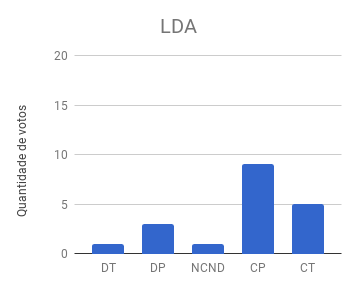
\includegraphics[width=.31\textwidth]{conteudo/capitulos/figs/figuras-experimento/C2-Q2-LDA.png}
%	}
%	\subfigure{ \label{fig:c2q2plsa}
		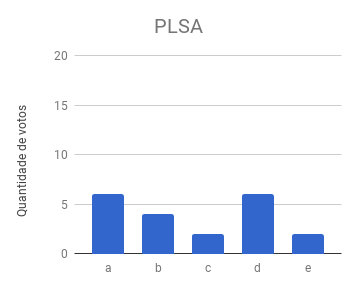
\includegraphics[width=.31\textwidth]{conteudo/capitulos/figs/figuras-experimento/C2-Q2-PLSA.png}
%	}

	\caption{Contagem das respostas referentes a Segunda questão. A primeira consulta, ``\textit{compra de equipamentos}'', é mostrada na linha superior e a segunda consulta, ``\textit{defesa de dissertação}'', na linha inferior.}
	\label{fig:c12-q2}
\end{figure}



% --> O K-means traz melhores segmentos (Sem misturar assuntos) em relação aos outros métodos.  'Aparentemente o K-means seleciona os trechos mais coesos, mas precisa de mais experimentos, mais amostras ...'





\section{Influência dos Extratores na qualidade dos segmentos}

A fim de analisar a influência das técnicas de extração de tópicos sobre a qualidade dos segmentos, quanto aos critérios de coesão e completude já mencionados. Vale lembrar que embora a extração de tópicos seja uma etapa posterior à extração, esta influencia na seleção dos segmentos apresentados ao usuário. 
A Figura~\ref{fig:influenciaExtSegQ3} apresenta as contagens das respostas da terceira questão, \textit{``Existem trechos que não tratam de um único assunto?''}, considerando-se cada extrator separadamente. De forma semelhante, a Figura~\ref{fig:influenciaExtSegQ4}, apresenta os dados da quarta resposta, \textit{``Existem trechos incompletos e insuficientes para compreensão do assunto do trecho?''}.



\begin{figure}[!h] \centering     %%% not \center

%	\subfigure{ \label{fig:t1q3}
		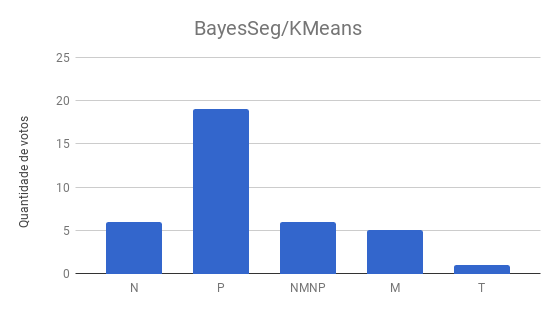
\includegraphics[width=.31\textwidth]{conteudo/capitulos/figs/figuras-experimento/t1q3.png}
%	}	
%	\subfigure{ \label{fig:t2q3}
		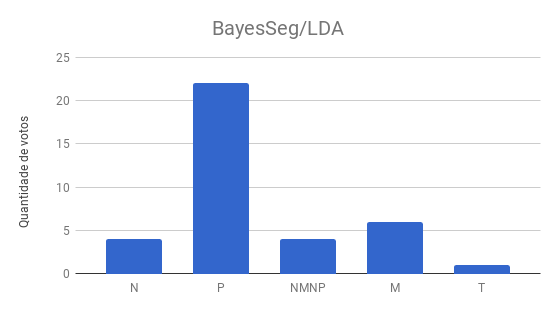
\includegraphics[width=.31\textwidth]{conteudo/capitulos/figs/figuras-experimento/t2q3.png}
%	}
%	\subfigure{ \label{fig:t3q3}
		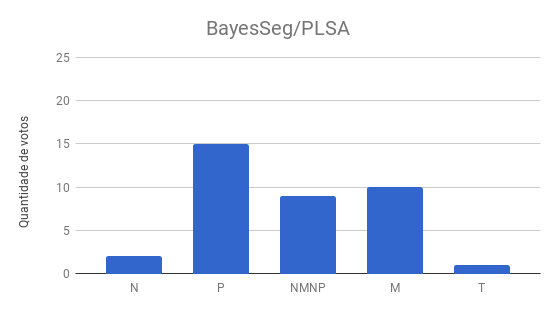
\includegraphics[width=.31\textwidth]{conteudo/capitulos/figs/figuras-experimento/t3q3.png}
%	}

	\caption{Contagem das respostas referentes a terceira questão, isolando-se as técnicas de extração de tópicos.}
	\label{fig:influenciaExtSegQ3}
\end{figure}

Verifica-se que os algoritmos K-Means e LDA selecionam segmentos igualmente coesos e pouco diferem entre si e em relação ao apresentado por todos os extratores, conforme mostrado na Figura~\ref{fig:Q3}, em que a maioria dos avaliadores informou que poucos segmentos não tratam de um único assunto. 
Sob o mesmo critério, os segmentos selecionados pelo PLSA são considerados menos coesos em relação aos demais modelos. 



% , segundo os avaliadores. 



\begin{figure}[!h] \centering     %%% not \center

%	\subfigure{ \label{fig:t1q4}
		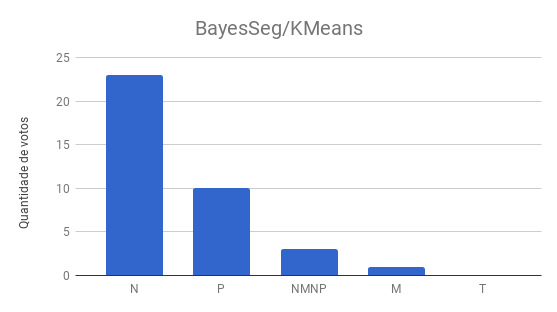
\includegraphics[width=.31\textwidth]{conteudo/capitulos/figs/figuras-experimento/t1q4.png}
%	}	
%	\subfigure{ \label{fig:t2q4}
		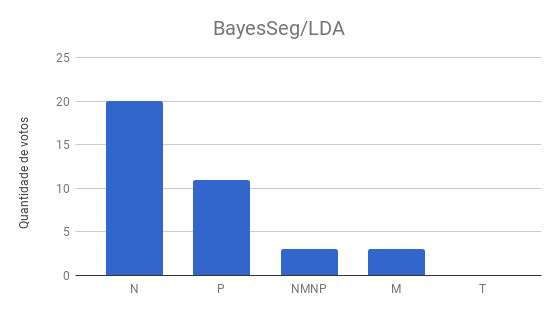
\includegraphics[width=.31\textwidth]{conteudo/capitulos/figs/figuras-experimento/t2q4.png}
%	}
%	\subfigure{ \label{fig:t3q4}
		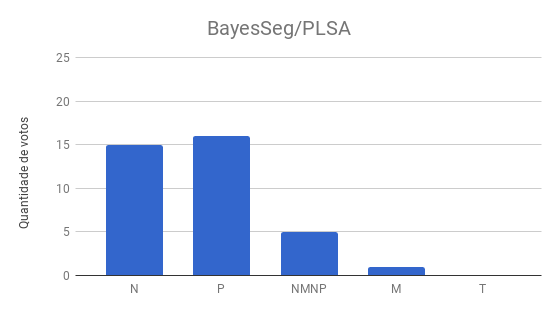
\includegraphics[width=.31\textwidth]{conteudo/capitulos/figs/figuras-experimento/t3q4.png}
%	}

	\caption{Contagem das respostas referentes a quarta questão, isolando-se as técnicas de extração de tópicos.}
	\label{fig:influenciaExtSegQ4}
\end{figure}


Quanto a completude dos segmentos selecionados por cada extrator, apresentados na Figura~\ref{fig:influenciaExtSegQ4}, observa-se um comportamento semelhante do extratores, sendo o K-Means e LDA semelhantes e com pouca discrepância em relação aos resultados analisados na Figura~\ref{fig:Q4}. O PLSA tente a tolerar segmentos menos coesos e menos completos enquanto os demais favorecem aqueles com maior qualidade de acordo com os quesitos abordados nesse experimento.




\section{Considerações finais}
% -- Conclusão : do conjunto das técnicas de extração e segmentação

Nessa seção, analisou-se a validação do BayesSeg como segmentador textual e as técnicas de extração de tópicos na criação de uma estrutura derivada do \textit{corpus} original como uma representação estruturada da coleção de atas a qual foi organizada e acrescida de atributos para sua descrição. As análises sugerem que tais técnicas podem oferecer a sistemas de recuperação uma representação estruturada que preserva o conteúdo dos documentos ao mesmo tempo que cria atributos adicionais que incorporam informação à base de dados e podem ser inseridas no espaço de busca.  

% Na maioria dos casos, os dados coletados apontam 


De maneira geral, os dados apontam que o modelo de K-Means como extrator de tópicos se sobressai em relação ao LDA e PLSA, sobre tudo quanto a sua eficiência em eleger bons descritores para representar os grupos, mostrando-se assim uma boa eficiência na tarefa de agrupar e descrever os segmentos.

Na validação do segmentador empregado no sistema, o \textit{BayesSeg}, consegue satisfazer os principais quesitos relacionados a um segmentador, contudo, o sistema apresenta resultados melhores quando selecionados por meio do K-Means e LDA, o que sugere que melhores configurações para o PLSA podem ser analisadas em outros experimentos.

% sendo menos eficiente quando selecionados por meio do PLSA

Os dados coletados forneceram uma base para as análises onde se verificou os pontos principais de cada técnica bem como a relação entre os modelos de extração de tópicos na seleção dos segmentos. Outros critérios podem ser levados em conta visto a subjetividade das avaliações bem como outros experimentos são necessários para averiguar o sistema na necessidade de análises mais profundas.

% podem ajudar a entender 
